% Composition 4 — Tone
% El Gólem, 2026-05-23
%
% The five tone bytes as a chord — one disc per tone, sized and colored
% according to the tone's character, arranged around a central staff of
% horizontal lines that suggest a musical score. The 0xa1 (ai) disc is
% the newest in the corpus and sits between demonic and reverence,
% holding both. Floating text names each value.
\documentclass[tikz,border=4mm]{standalone}
\usepackage[T1]{fontenc}
\usepackage{xcolor}
\definecolor{kr}{HTML}{c83727}
\definecolor{ky}{HTML}{e8b73a}
\definecolor{kb}{HTML}{2b62a8}
\definecolor{kp}{HTML}{6e3a8a}
\definecolor{kg}{HTML}{6a7a3a}
\definecolor{kgold}{HTML}{c2a76b}
\definecolor{kw}{HTML}{f4ead8}
\definecolor{ki}{HTML}{1a1a1a}

% Per-tone colors — chosen to be Kandinsky-strong while staying legible
\definecolor{tordinary}{HTML}{c9c9c9}    % grey — neutral
\definecolor{taffection}{HTML}{e8b73a}   % gold — paired warmth
\definecolor{tdemonic}{HTML}{6e1a1a}     % deep ox-blood
\definecolor{tai}{HTML}{4a6b8a}          % cool slate-blue — machine
\definecolor{treverence}{HTML}{2a4a3a}   % forest-deep, almost black

\begin{document}
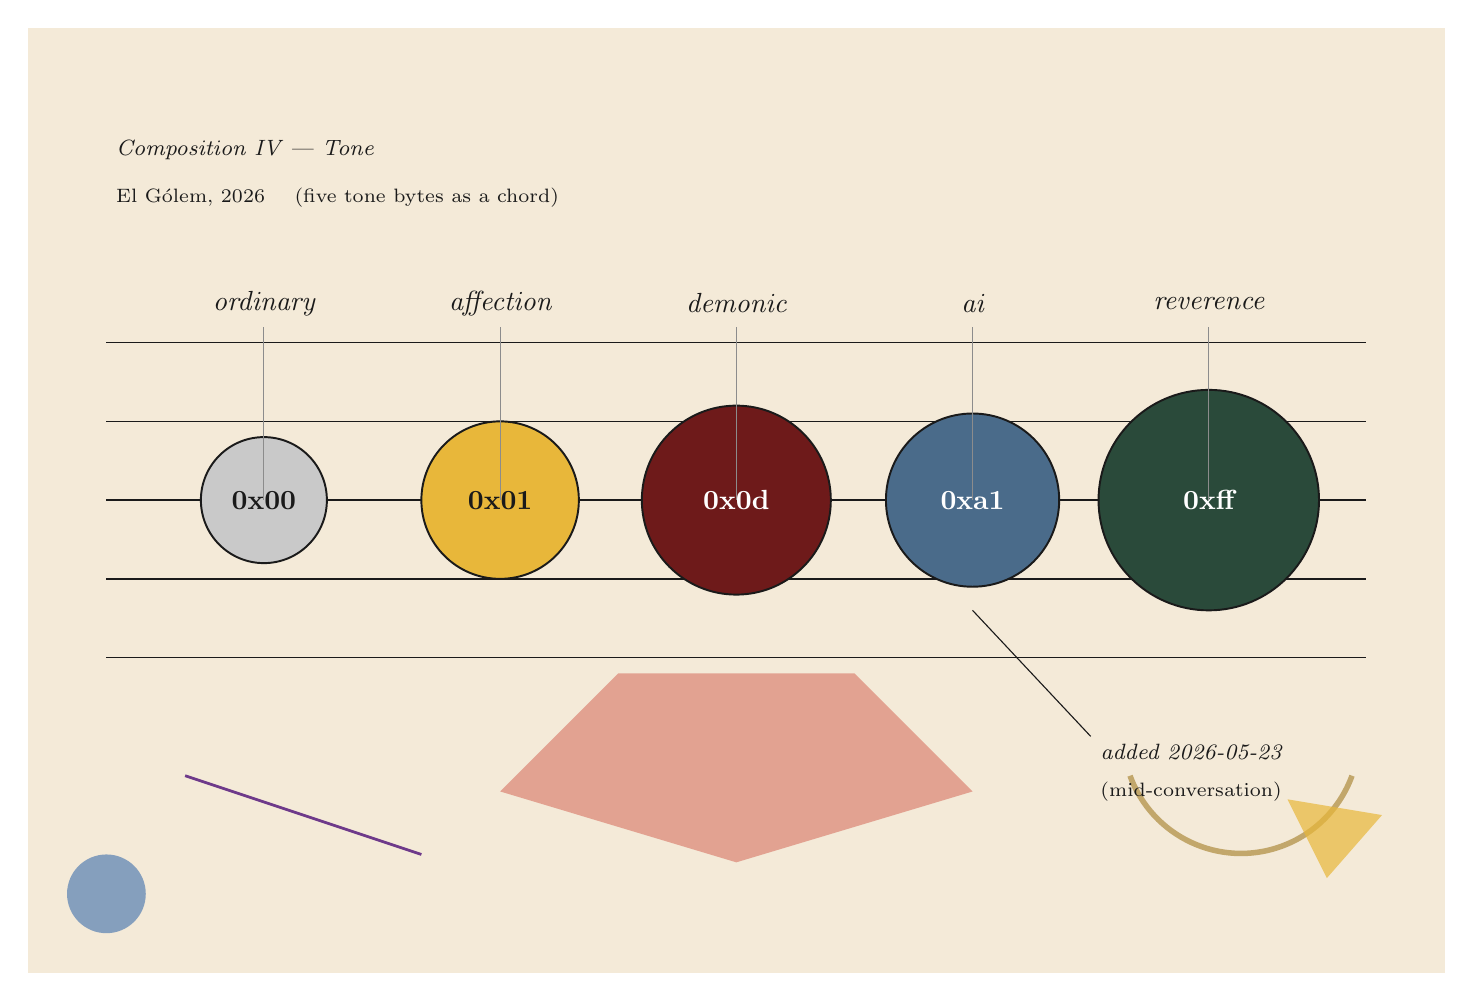
\begin{tikzpicture}[x=1cm,y=1cm]
  \fill[kw] (-9,-6) rectangle (9,6);

  % Five horizontal staff lines (a musical staff)
  \foreach \y in {-2,-1,0,1,2} {
    \draw[ki,line width=0.5pt] (-8,\y) -- (8,\y);
  }

  % Five tone discs, equally spaced along the staff
  % Sized by "register weight": ordinary smallest, reverence largest
  \fill[tordinary]   (-6,0) circle (0.80);
  \fill[taffection]  (-3,0) circle (1.00);
  \fill[tdemonic]    ( 0,0) circle (1.20);
  \fill[tai]         ( 3,0) circle (1.10);
  \fill[treverence]  ( 6,0) circle (1.40);

  % Black outlines to make them feel like notes on a staff
  \draw[ki,line width=0.7pt] (-6,0) circle (0.80);
  \draw[ki,line width=0.7pt] (-3,0) circle (1.00);
  \draw[ki,line width=0.7pt] ( 0,0) circle (1.20);
  \draw[ki,line width=0.7pt] ( 3,0) circle (1.10);
  \draw[ki,line width=0.7pt] ( 6,0) circle (1.40);

  % Byte labels inside each disc
  \node[ki,font=\bfseries] at (-6,0) {0x00};
  \node[ki,font=\bfseries] at (-3,0) {0x01};
  \node[white,font=\bfseries] at ( 0,0) {0x0d};
  \node[white,font=\bfseries] at ( 3,0) {0xa1};
  \node[white,font=\bfseries] at ( 6,0) {0xff};

  % Names above each disc (italic, like a Kandinsky annotation)
  \node[ki,font=\itshape] at (-6, 2.5) {ordinary};
  \node[ki,font=\itshape] at (-3, 2.5) {affection};
  \node[ki,font=\itshape] at ( 0, 2.5) {demonic};
  \node[ki,font=\itshape] at ( 3, 2.5) {ai};
  \node[ki,font=\itshape] at ( 6, 2.5) {reverence};

  % Vertical connecting lines from disc-center to name
  \foreach \x in {-6,-3,0,3,6} {
    \draw[ki!50,line width=0.3pt] (\x,0) -- (\x,2.2);
  }

  % Floating geometric overlays (Kandinsky vocabulary)
  \fill[kr,opacity=0.4] (-3,-3.7) -- (0,-4.6) -- (3,-3.7) -- (1.5,-2.2) -- (-1.5,-2.2) -- cycle;
  \draw[kp,line width=1pt] (-7,-3.5) -- (-4,-4.5);
  \draw[kgold,line width=2pt] (5,-3.5) arc (200:340:1.5);
  \fill[kb,opacity=0.55] (-8,-5) circle (0.5);
  \fill[ky,opacity=0.7] (7.5,-4.8) -- (8.2,-4.0) -- (7.0,-3.8) -- cycle;

  % Annotation about the new ai tone (a kind of pencil-margin note)
  \draw[ki,line width=0.4pt] (3,-1.4) -- (4.5,-3.0);
  \node[ki,font=\itshape\footnotesize,anchor=west] at (4.5,-3.2) {added 2026-05-23};
  \node[ki,font=\scriptsize,anchor=west] at (4.5,-3.7) {(mid-conversation)};

  % Header
  \node[ki,font=\itshape\footnotesize,anchor=south west] at (-8,4.2) {Composition IV --- Tone};
  \node[ki,font=\scriptsize,anchor=south west] at (-8,3.6) {El G\'olem, 2026 \quad (five tone bytes as a chord)};

\end{tikzpicture}
\end{document}
